\title[Parasitics and PCB layout]{Parasitics and PCB layout}
\section{Parasitics and PCB layout}

\begin{frame}[plain]
	\titlepage
\end{frame}

%%%%%%%%%%%%%%%%%%%%%%%%%%%%%%%%%%%%%%%%%%%%%%%%%%%%%%%%%%%%%
%% Overview %%
%%%%%%%%%%%%%%%%%%%%%%%%%%%%%%%%%%%%%%%%%%%%%%%%%%%%%%%%%%%%%
\subsection{Commutation loops}

\begin{frame}
	\frametitle{Overview}
	Lecture 2 treated the switching cell as a set of ideal connections. At several MHz, with current slopes of amperes per nanosecond, the copper between the parts becomes part of the circuit.
	\begin{itemize}
		\item Which loops matter: power loop, gate loop and their common part
		\item How to estimate inductance and capacitance of a layout with pencil and paper
		\item Consequences: ringing, overshoot, extra loss and false turn-on
		\item Layout rules for a GaN half-bridge
		\item Damping with an RC snubber, and when not to use one
	\end{itemize}
	After this lecture you can estimate the loop inductance of a layout, predict the ringing it causes and lay out a half-bridge power stage.
\end{frame}

%%%%%%%%%%%%%%%%%%%%%%%%%%%%%%%%%%%%%%%%%%%%%%%%%%%%%%%%%%%%%
%% Loops of a half-bridge %%
%%%%%%%%%%%%%%%%%%%%%%%%%%%%%%%%%%%%%%%%%%%%%%%%%%%%%%%%%%%%%
\begin{frame}
	\frametitle{Loops of a half-bridge}
	\begin{columns}[T]
		\begin{column}{0.5\textwidth}
			\begin{figure}
				\centering
				\begin{circuitikz}[scale=0.7, transform shape]
					% input capacitor with its mounting inductance, drain-side inductance
					\draw (0,-1.9) to[C, l=$C_\mathrm{in}$] (0,0.9) to[L, l=$L_\mathrm{C}$] (0,3.4) -- (0.3,3.4) to[L, l=$L_\mathrm{D}$] (2.3,3.4) -- (3.0,3.4);
					% high-side and low-side switch, both with the gate on the right
					\draw (3.0,3.4) node[nigfete, anchor=D, xscale=-1](Q1){};
					\draw (Q1.S) -- ++(0,-0.35) coordinate (sw);
					\draw (sw) node[nigfete, anchor=D, xscale=-1](Q2){};
					\draw (Q2.S) to[L, l=$L_\mathrm{CS}$] ++(0,-1.4) coordinate (k) -- ++(0,-0.45) coordinate (pg);
					\draw (pg) -- (0,-1.9 |- pg) -- (0,-1.9);
					\draw (Q1.G) -- ++(0.3,0) node[right]{\footnotesize to HS driver};
					% switch node and load current
					\draw (sw) node[circ]{} -- ++(1.5,0) to[short, i=$I_\mathrm{L}$] ++(1.0,0) node[right]{to $L_\mathrm{o}$};
					% low-side gate loop, driver return at the power ground below L_CS
					\draw (Q2.G) -- ++(0.7,0) coordinate (g) to[R, l=$R_\mathrm{G}$] ++(0,-1.1) coordinate (d) to[sV, l=driver] (d |- pg) -- (pg);
					\draw (pg) node[circ]{};
					% loop markers
					\draw[densely dashed, rounded corners=4pt, -{Latex[length=2mm]}] (2.2,-1.35) -- (0.6,-1.35) -- (0.6,2.85) -- (2.2,2.85);
					\node[align=center, font=\small] at (1.55,0.7) {power\\loop};
				\end{circuitikz}
				\caption{Half-bridge with the inductances of the power loop; low-side gate loop: $R_\mathrm{G}$, driver, $L_\mathrm{CS}$}
			\end{figure}
		\end{column}
		\begin{column}{0.47\textwidth}
			\small
			\begin{itemize}
				\item \textbf{Power loop}: $C_\mathrm{in}$, high-side and low-side switch. Its current changes by $I_\mathrm{L}$ at every transition. $L_\mathrm{loop}=L_\mathrm{C}+L_\mathrm{D}+L_\mathrm{CS}+\ldots$ (packages, pads, vias, planes).
				\item \textbf{Gate loop}: driver, gate, source and back.
				\item \textbf{Common-source inductance} $L_\mathrm{CS}$: the part shared by both loops (L2).
			\end{itemize}
			Order of importance for the layout: $L_\mathrm{CS}$, then the power loop, then the gate loop.\\[0.4em]
			At high frequency the loop is closed by small ceramic capacitors next to the switches, not by the bulk capacitor.
		\end{column}
	\end{columns}
	\blfootnote{Source: Lidow et al., GaN Transistors for Efficient Power Conversion, 3rd ed., 2019, Sec. 4.1--4.2.}
\end{frame}

%%%%%%%%%%%%%%%%%%%%%%%%%%%%%%%%%%%%%%%%%%%%%%%%%%%%%%%%%%%%%
%% Six parasitics %%
%%%%%%%%%%%%%%%%%%%%%%%%%%%%%%%%%%%%%%%%%%%%%%%%%%%%%%%%%%%%%
\begin{frame}
	\frametitle{Parasitic elements of one switch}
	\begin{columns}[T]
		\begin{column}{0.44\textwidth}
			\begin{figure}
				\centering
				\begin{circuitikz}[scale=0.68, transform shape]
					\draw (2.6,1.6) node[nigfete](Q){};
					\draw (Q.D) -- ++(0,0.6) coordinate (d0);
					\draw (Q.S) -- ++(0,-0.6) coordinate (s0);
					\draw (Q.G) -- ++(-1.0,0) coordinate (g0);
					\draw (g0) to[C, l_=$C_\mathrm{gd}$, *-] (g0 |- d0) -- (d0);
					\draw (g0) to[C, l=$C_\mathrm{gs}$] (g0 |- s0) -- (s0);
					\draw (d0) -- ++(1.2,0) coordinate (dr) to[C, l=$C_\mathrm{ds}$] (dr |- s0) -- (s0);
					\draw (d0) node[circ]{} to[L, l_=$L_\mathrm{ds}$] ++(0,1.5) node[above]{to $C_\mathrm{in}$};
					\draw (s0) node[circ]{} to[L, l_=$L_\mathrm{cm}$] ++(0,-1.5) coordinate (k) node[circ]{} -- ++(0,-0.3) node[below]{power ground};
					\draw (g0) to[L, l_=$L_\mathrm{gs}$] ++(-1.5,0) to[R, l_=$R_\mathrm{G}$] ++(-1.5,0) coordinate (dv) to[sV, l_=driver] (dv |- k) -- (k);
				\end{circuitikz}
				\caption{Switch in a phase leg: die capacitances inside, layout inductances outside}
			\end{figure}
		\end{column}
		\begin{column}{0.53\textwidth}
			\begin{table}
				\centering
				\footnotesize
				\begin{tabular}{|l|l|>{\raggedright\arraybackslash}p{4.5cm}|}
					\hline
					\textbf{Element}   & \textbf{Loop}   & \textbf{Effect}                                                 \\
					\hline
					$L_\mathrm{ds}$    & power           & overshoot, ringing, $\frac12LI^2$ per turn-off                  \\
					$C_\mathrm{ds}$    & power           & ringing frequency, $Q_\mathrm{oss}V$ loss                        \\
					$L_\mathrm{gs}$    & gate            & gate ringing, slower gate current                                \\
					$C_\mathrm{gs}$    & gate            & stores the gate charge                                           \\
					$L_\mathrm{cm}$    & both            & feeds $\mathrm{d}i/\mathrm{d}t$ back into the gate loop: slower switching \\
					$C_\mathrm{gd}$    & both            & feeds $\mathrm{d}v/\mathrm{d}t$ back: slower switching, false turn-on \\
					\hline
				\end{tabular}
				\caption{$L_\mathrm{ds}$: all inductance of the power loop; $C_\mathrm{ds}$: all capacitance across the switch. The mutual elements couple the power loop into the gate loop.}
			\end{table}
		\end{column}
	\end{columns}
	\blfootnote{Source: Zhang, Guo, Wang, Tolbert, Blalock, Liang, Ning, IEEE APEC 2014, pp.\ 2534--2541.}
\end{frame}

%%%%%%%%%%%%%%%%%%%%%%%%%%%%%%%%%%%%%%%%%%%%%%%%%%%%%%%%%%%%%
%% Inductance of a loop %%
%%%%%%%%%%%%%%%%%%%%%%%%%%%%%%%%%%%%%%%%%%%%%%%%%%%%%%%%%%%%%
\begin{frame}
	\frametitle{Inductance of a loop}
	\begin{columns}[T]
		\begin{column}{0.44\textwidth}
			\begin{figure}
				\centering
				\begin{tikzpicture}[font=\scriptsize]
					% (a) conductors far apart
					\foreach \r in {0.3,0.5,0.72} {\draw[gray] (0,0) circle (\r); \draw[gray] (2.0,0) circle (\r);}
					\filldraw[fill=white] (0,0) circle (0.14); \fill (0,0) circle (0.04);
					\filldraw[fill=white] (2.0,0) circle (0.14);
					\draw (2.0,0) ++(-0.09,-0.09) -- ++(0.18,0.18) ++(0,-0.18) -- ++(-0.18,0.18);
					\node at (1.0,-1.1) {(a) far apart};
					% (b) close strips
					\fill[gray!60] (3.2,0.1) rectangle (5.4,0.22);
					\fill[gray!60] (3.2,-0.22) rectangle (5.4,-0.1);
					\foreach \x in {3.4,3.85,4.3,4.75} {\draw[gray, -{Latex[length=1.2mm]}] (\x,0) -- ++(0.32,0);}
					\node[anchor=south] at (4.3,0.25) {$+I$};
					\node[anchor=north] at (4.3,-0.25) {$-I$};
					\node at (4.3,-1.1) {(b) close together};
				\end{tikzpicture}
				\caption{Go and return conductor in cross-section; (b): the field is confined to the gap}
			\end{figure}
			\begin{block}{Key message}
				Forward and return current as close together as possible; wide and short paths.
			\end{block}
		\end{column}
		\begin{column}{0.53\textwidth}
			\small
			\begin{itemize}
				\item Inductance belongs to a closed loop: $L_\mathrm{loop}=\Phi/I$, the flux through the loop per ampere.
				\item The stored energy is in the field:
				      \begin{equation*}
					      \tfrac12 L_\mathrm{loop}I^2=\int\frac{B^2}{2\mu_0}\,\mathrm{d}V
				      \end{equation*}
				      Less volume with field, less inductance.
				\item \textbf{Partial inductance} assigns shares to segments. For a go and return conductor
				      \begin{equation*}
					      L_\mathrm{loop}=L_\mathrm{p1}+L_\mathrm{p2}-2M_\mathrm{p12}
				      \end{equation*}
				      Close conductors with opposite currents have a large $M_\mathrm{p12}$, which cancels most of the self terms.
			\end{itemize}
		\end{column}
	\end{columns}
	\blfootnote{Source: Ott, Electromagnetic Compatibility Engineering, Wiley, 2009, App.\ E.}
\end{frame}

%%%%%%%%%%%%%%%%%%%%%%%%%%%%%%%%%%%%%%%%%%%%%%%%%%%%%%%%%%%%%
%% Estimating parasitics %%
%%%%%%%%%%%%%%%%%%%%%%%%%%%%%%%%%%%%%%%%%%%%%%%%%%%%%%%%%%%%%
\subsection{Estimating parasitics}

\begin{frame}
	\frametitle{Parallel planes}
	\begin{columns}[T]
		\begin{column}{0.5\textwidth}
			\begin{figure}
				\centering
				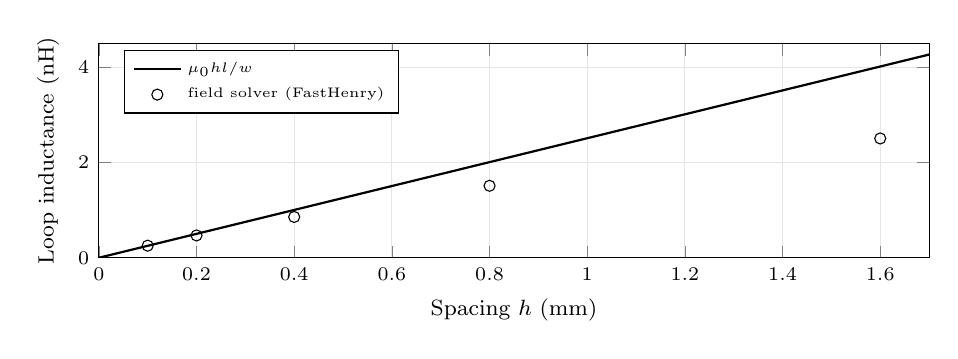
\begin{tikzpicture}
					\begin{axis}[
							width=\linewidth, height=4.3cm,
							xmin=0, xmax=1.7, ymin=0, ymax=4.5,
							xlabel={Spacing $h$ (mm)}, ylabel={Loop inductance (nH)},
							grid=major, grid style={gray!20},
							tick label style={font=\scriptsize}, label style={font=\footnotesize},
							legend style={font=\tiny}, legend pos=north west, legend cell align=left,
						]
						\addplot[black, thick, domain=0:1.7, samples=2] {2.513*x};
						\addlegendentry{$\mu_0hl/w$}
						\addplot[black, only marks, mark=o, mark size=2pt] coordinates {(0.1,0.254) (0.2,0.469) (0.4,0.858) (0.8,1.513) (1.6,2.508)};
						\addlegendentry{field solver (FastHenry)}
					\end{axis}
				\end{tikzpicture}
				\caption{Two copper strips with opposite currents, $w=5$\,mm, $l=10$\,mm, 100\,MHz}
			\end{figure}
		\end{column}
		\begin{column}{0.47\textwidth}
			\small
			Two planes of width $w$ and length $l$, spacing $h\ll w$; the field is confined to the gap:
			\begin{equation*}
				L\approx\mu_0\frac{h\,l}{w}=1.26\,\frac{\mathrm{nH}}{\mathrm{mm}}\cdot\frac{h\,l}{w}
			\end{equation*}
			\begin{itemize}
				\item $h=0.1$\,mm: 0.25\,nH, as the solver.
				\item $h=1.6$\,mm: formula 4.0\,nH, solver 2.5\,nH; at $w/h\approx3$ the field spreads beyond the edges.
			\end{itemize}
			\begin{block}{Key message}
				Return on the adjacent layer: ten times less inductance than across a 1.6\,mm board.
			\end{block}
		\end{column}
	\end{columns}
	\blfootnote{Formula: Lidow et al., 2019, Eq.\ (4.1). Solver results: FastHenry 3.0, computed for this lecture.}
\end{frame}

%%%%%%%%%%%%%%%%%%%%%%%%%%%%%%%%%%%%%%%%%%%%%%%%%%%%%%%%%%%%%
%% Vias and wires %%
%%%%%%%%%%%%%%%%%%%%%%%%%%%%%%%%%%%%%%%%%%%%%%%%%%%%%%%%%%%%%
\begin{frame}
	\frametitle{Vias and wires}
	Partial inductance of a straight round conductor, length $l$, diameter $d$ ($l\gg d$, current at the surface):
	\begin{equation*}
		L_\mathrm{p}\approx\frac{\mu_0 l}{2\pi}\left[\ln\frac{4l}{d}-1\right]=0.2\,\frac{\mathrm{nH}}{\mathrm{mm}}\cdot l\left[\ln\frac{4l}{d}-1\right]
	\end{equation*}
	\begin{columns}[T]
		\begin{column}{0.48\textwidth}
			\centering
			\small
			\begin{tabular}{|l|r|}
				\hline
				\multicolumn{2}{|l|}{\textbf{Partial self-inductance}} \\
				\hline
				via, $l=1.6$\,mm, $d=0.3$\,mm      & 0.7\,nH \\
				bond wire, 2\,mm, 25\,$\mu$m        & 1.9\,nH \\
				wire, 10\,mm, 0.5\,mm              & 6.8\,nH \\
				\hline
			\end{tabular}\\[0.6em]
			\raggedright
			Rule of thumb for thin wires: about 1\,nH per mm.
		\end{column}
		\begin{column}{0.48\textwidth}
			\centering
			\small
			\begin{tabular}{|l|r|}
				\hline
				\multicolumn{2}{|l|}{\textbf{Loop, 1.6\,mm vias, 1\,mm pitch}} \\
				\hline
				1 via pair                         & 1.06\,nH \\
				2 pairs, interleaved               & 0.49\,nH \\
				4 pairs, interleaved               & 0.24\,nH \\
				\hline
			\end{tabular}\\[0.6em]
			\raggedright
			Interleaved forward and return vias act in parallel and cancel each other's field (FastHenry, 100\,MHz).
		\end{column}
	\end{columns}
	\blfootnote{Source: Ott, 2009, Eq.\ (E-14), after Grover, 1946. The often quoted $5.08\,h\,[\ln(4h/d)+1]$\,nH ($h,d$ in inch) gives 1.3\,nH for the via, 1.8 times the solver value.}
\end{frame}

%%%%%%%%%%%%%%%%%%%%%%%%%%%%%%%%%%%%%%%%%%%%%%%%%%%%%%%%%%%%%
%% Spot the loop %%
%%%%%%%%%%%%%%%%%%%%%%%%%%%%%%%%%%%%%%%%%%%%%%%%%%%%%%%%%%%%%
% Two pages: question (page 1) and answer (page 2).
\begin{frame}<handout:1-2>
	\frametitle{Spot the loop}
	Both power loops use 4\,mm wide copper and four vias at each end. Which one has the lower loop inductance? Vote.
	\begin{figure}
		\centering
		\begin{tikzpicture}[x=0.55cm, y=1cm, font=\scriptsize]
			% layout A: 10 mm loop, plane 0.1 mm below
			\fill[gray!15] (-1.6,-0.1) rectangle (11.4,0.0);
			\fill[gray!60] (-1.6,-0.17) rectangle (11.4,-0.1);
			\fill[gray!60] (0,0) rectangle (10,0.07);
			\fill[gray!60] (-1.2,0) rectangle (-0.4,0.07);
			\draw[thick] (9.6,0.07) -- (9.6,-0.1);
			\draw[thick] (-0.8,0.07) -- (-0.8,-0.1);
			\draw[-{Latex[length=1.6mm]}] (0.5,0.25) -- (9,0.25);
			\draw[-{Latex[length=1.6mm]}] (9,-0.4) -- (0.5,-0.4);
			\node[anchor=south] at (-0.8,0.1) {$C_\mathrm{in}$};
			\node[anchor=south] at (10.2,0.1) {switches};
			\node[anchor=north] at (5,-0.45) {return on the first inner layer, 0.1\,mm below};
			\node[anchor=east] at (-2.0,0) {\small\textbf{A}};
			% layout B: 3 mm loop, plane 1.6 mm below
			\begin{scope}[xshift=8.6cm]
				\fill[gray!15] (-1.6,-1.6) rectangle (4.6,0.0);
				\fill[gray!60] (-1.6,-1.67) rectangle (4.6,-1.6);
				\fill[gray!60] (0,0) rectangle (3,0.07);
				\fill[gray!60] (-1.2,0) rectangle (-0.4,0.07);
				\draw[thick] (2.6,0.07) -- (2.6,-1.6);
				\draw[thick] (-0.8,0.07) -- (-0.8,-1.6);
				\draw[-{Latex[length=1.6mm]}] (0.2,0.25) -- (2.4,0.25);
				\draw[-{Latex[length=1.6mm]}] (2.4,-1.9) -- (0.2,-1.9);
				\node[anchor=south] at (-0.8,0.1) {$C_\mathrm{in}$};
				\node[anchor=south] at (3.0,0.1) {switches};
				\node[anchor=north] at (1.5,-1.95) {return on the bottom layer, 1.6\,mm below};
				\node[anchor=east] at (-2.0,0) {\small\textbf{B}};
			\end{scope}
		\end{tikzpicture}
		\caption{Side views; A: loop 10\,mm long, B: loop 3\,mm long (vertical scale 1.8 times the horizontal)}
	\end{figure}
	\onslide<2-|handout:2>{
		\begin{block}{Answer: A}
			FastHenry at 100\,MHz: A 0.47\,nH, B 1.4\,nH. What counts is the area between forward and return current, $10\cdot0.1=1\,\mathrm{mm^2}$ for A and $3\cdot1.6=4.8\,\mathrm{mm^2}$ for B, not the length of the loop.
		\end{block}
	}
\end{frame}

%%%%%%%%%%%%%%%%%%%%%%%%%%%%%%%%%%%%%%%%%%%%%%%%%%%%%%%%%%%%%
%% Switch-node capacitance %%
%%%%%%%%%%%%%%%%%%%%%%%%%%%%%%%%%%%%%%%%%%%%%%%%%%%%%%%%%%%%%
\begin{frame}
	\frametitle{Switch-node capacitance}
	\begin{columns}[T]
		\begin{column}{0.5\textwidth}
			\begin{figure}
				\centering
				\begin{tikzpicture}[font=\scriptsize]
					% board (not to scale)
					\fill[gray!15] (0,0) rectangle (5.0,2.0);
					\fill[gray!60] (0,1.2) rectangle (5.0,1.28);
					\node[anchor=west] at (5.05,1.24) {L2: PGND};
					% switch-node copper on top and bottom, thermal vias
					\fill[gray!60] (1.3,2.0) rectangle (3.7,2.08);
					\fill[gray!60] (1.3,-0.08) rectangle (3.7,0);
					\foreach \x in {1.7,2.2,2.7,3.2} {\fill[gray!60] (\x,0) rectangle ++(0.1,2.0);}
					% device
					\draw[fill=white] (1.8,2.08) rectangle (3.2,2.45);
					\node at (2.5,2.27) {GaN};
					\node[anchor=west] at (3.75,2.25) {switch node};
					% thermal interface and heat sink
					\fill[gray!30] (1.0,-0.68) rectangle (4.0,-0.08);
					\draw[fill=gray!45] (0,-1.25) rectangle (5.0,-0.68);
					\node at (2.5,-0.965) {heat sink (earthed)};
					\node[anchor=west] at (5.05,-0.38) {thermal interface};
					% capacitances
					\begin{scope}[circuitikz/bipoles/length=0.75cm]
						\draw[densely dashed] (1.3,2.04) -- (0.6,2.04);
						\draw (0.6,2.04) to[C, l_=$C_1$] (0.6,1.28);
						\draw[densely dashed] (3.7,-0.04) -- (4.5,-0.04);
						\draw (4.5,-0.04) to[C, l_=$C_2$] (4.5,-0.68);
					\end{scope}
				\end{tikzpicture}
				\caption{High-side switch: its source is the switch node (not to scale)}
			\end{figure}
		\end{column}
		\begin{column}{0.47\textwidth}
			\small
			Parallel-plate estimate $C=\varepsilon_0\varepsilon_\mathrm{r}A/h$:
			\begin{itemize}
				\item $C_1$: 10\,mm $\times$ 10\,mm over PGND at 0.1\,mm, FR-4 ($\varepsilon_\mathrm{r}\approx4.4$): 39\,pF
				\item $C_2$: 30\,mm$^2$ on a 0.2\,mm thermal interface ($\varepsilon_\mathrm{r}\approx5$): 7\,pF
			\end{itemize}
			Consequences at every edge:
			\begin{itemize}
				\item $C_1$ adds to $C_\mathrm{oss}$: extra hard-switching loss $\frac12C_1V^2f_\mathrm{sw}$, 0.045\,W at 48\,V but 3.1\,W at 400\,V (1\,MHz)
				\item $C_2$ to earth: common-mode current $C_2\,\mathrm{d}v/\mathrm{d}t$, 0.7\,A at 100\,V/ns, a main source of common-mode EMI (L14)
			\end{itemize}
			Rule of thumb: 10\,pF at 100\,V/ns give 1\,A.
		\end{column}
	\end{columns}
\end{frame}

%%%%%%%%%%%%%%%%%%%%%%%%%%%%%%%%%%%%%%%%%%%%%%%%%%%%%%%%%%%%%
%% Capacitor mounting %%
%%%%%%%%%%%%%%%%%%%%%%%%%%%%%%%%%%%%%%%%%%%%%%%%%%%%%%%%%%%%%
\begin{frame}
	\frametitle{Capacitor mounting}
	\begin{columns}[T]
		\begin{column}{0.46\textwidth}
			\begin{figure}
				\centering
				\begin{tikzpicture}[font=\scriptsize, scale=1.15]
					\fill[gray!15] (0,0) rectangle (5,0.9);
					\fill[gray!60] (0,0.62) rectangle (5,0.7);
					\node[anchor=west] at (5.05,0.66) {L2};
					% pads and capacitor body
					\fill[gray!60] (1.0,0.9) rectangle (1.8,0.98);
					\fill[gray!60] (3.2,0.9) rectangle (4.0,0.98);
					\draw[fill=white] (1.2,0.98) rectangle (3.8,1.6);
					\foreach \x in {1.5,1.8,...,3.5} {\draw[gray] (\x,1.05) -- (\x,1.53);}
					\node[anchor=south] at (2.5,1.62) {MLCC};
					% via to the plane at the right pad
					\fill[gray!60] (3.55,0.62) rectangle (3.65,0.9);
					% current path
					\draw[-{Latex[length=1.5mm]}] (0.2,1.12) -- (1.0,1.12) -- (1.15,1.3);
					\draw[-{Latex[length=1.5mm]}] (3.6,0.9) -- (3.6,0.45);
					\draw[-{Latex[length=1.5mm]}] (3.4,0.45) -- (0.3,0.45);
					\node[anchor=north] at (2.5,0.0) {current: pad, body, via, plane};
				\end{tikzpicture}
				\caption{Decoupling capacitor in the power loop (side view)}
			\end{figure}
		\end{column}
		\begin{column}{0.51\textwidth}
			\small
			Inductance in series with a decoupling capacitor: the body (ESL in the datasheet, measured on the vendor's fixture), pads, traces and vias, and current spreading in the planes. The body is usually the smallest part.
			\begin{itemize}
				\item vias at or in the pads, return plane on the adjacent layer
				\item several small capacitors in parallel, each with its own vias
				\item reverse geometry (terminals on the long side, e.g.\ 0306 instead of 0603): 50--80\,\% lower ESL according to manufacturers
			\end{itemize}
		\end{column}
	\end{columns}
	\blfootnote{Sources: Ott, 2009, Sec.\ 11.3; manufacturer information on reverse-geometry MLCCs (Yageo, NIC Components).}
\end{frame}

%%%%%%%%%%%%%%%%%%%%%%%%%%%%%%%%%%%%%%%%%%%%%%%%%%%%%%%%%%%%%
%% Tool chain %%
%%%%%%%%%%%%%%%%%%%%%%%%%%%%%%%%%%%%%%%%%%%%%%%%%%%%%%%%%%%%%
\begin{frame}
	\frametitle{From estimate to field solver}
	\begin{table}
		\centering
		\small
		\begin{tabular}{|>{\raggedright\arraybackslash}p{3.0cm}|>{\raggedright\arraybackslash}p{4.6cm}|>{\raggedright\arraybackslash}p{4.8cm}|}
			\hline
			\textbf{Step}                & \textbf{Tool}                                             & \textbf{Use}                                                   \\
			\hline
			Hand estimate                & formulas of this lecture                                  & stack-up and placement                                         \\
			Quasi-static field solver    & FastHenry (inductance), FasterCap (capacitance), both open source; Ansys Q3D & values of the routed layout              \\
			Circuit simulation           & SPICE with device models and extracted parasitics         & ringing, overshoot, losses                                     \\
			Measurement                  & ringing frequency, double-pulse test                      & check of the extracted values (L5)                             \\
			\hline
		\end{tabular}
	\end{table}
	\begin{itemize}
		\item Extract at the ringing frequency (100\,MHz to 1\,GHz): the current flows on the facing copper surfaces.
		\item Device models contain no layout inductance. Add it in SPICE together with a resistance that represents the damping at $f_\mathrm{r}$ (skin effect, capacitor ESR).
	\end{itemize}
	\blfootnote{Sources: Kamon, Tsuk, White, IEEE Trans.\ MTT, vol.\ 42, no.\ 9, 1994 (FastHenry); Lidow et al., 2019, Sec.\ 5.2.}
\end{frame}

%%%%%%%%%%%%%%%%%%%%%%%%%%%%%%%%%%%%%%%%%%%%%%%%%%%%%%%%%%%%%
%% Consequences %%
%%%%%%%%%%%%%%%%%%%%%%%%%%%%%%%%%%%%%%%%%%%%%%%%%%%%%%%%%%%%%
\subsection{Consequences}

\begin{frame}
	\frametitle{Ringing of the power loop}
	\begin{columns}[T]
		\begin{column}{0.5\textwidth}
			\begin{figure}
				\centering
				\begin{tikzpicture}
					\begin{axis}[
							width=\linewidth, height=4.6cm,
							xmin=-1, xmax=10, ymin=-5, ymax=95,
							xlabel={$t$ (ns)}, ylabel={$v_\mathrm{sw}$ (V)},
							grid=major, grid style={gray!20},
							tick label style={font=\scriptsize}, label style={font=\footnotesize},
						]
						\addplot[black, thick] table[x=t, y=v16] {fig/lec03/ring_turn_on.dat};
						\addplot[black, densely dotted, domain=-1:10, samples=2] {48};
						\draw[{Latex[length=1.5mm]}-{Latex[length=1.5mm]}] (axis cs:2.55,89) -- (axis cs:6.6,89) node[midway, below, font=\scriptsize] {$T_\mathrm{r}=1/f_\mathrm{r}$};
					\end{axis}
				\end{tikzpicture}
				\caption{Hard turn-on, switch-node voltage; 48\,V, $L_\mathrm{loop}=1.6$\,nH, $C=260$\,pF, $t_\mathrm{r}=1$\,ns (model)}
			\end{figure}
		\end{column}
		\begin{column}{0.47\textwidth}
			\small
			Every transition excites the series resonance of $L_\mathrm{loop}$ with the capacitance across the switch that is off:
			\begin{equation*}
				f_\mathrm{r}=\frac{1}{2\pi\sqrt{L_\mathrm{loop}C}},\quad Z_0=\sqrt{\frac{L_\mathrm{loop}}{C}}
			\end{equation*}
			with $C=C_\mathrm{oss}(V_\mathrm{DC})+C_\mathrm{par}$ (small-signal value, plus layout and probe).
			\begin{itemize}
				\item 1\,nH and 250\,pF: $f_\mathrm{r}=318$\,MHz, $Z_0=2\,\Omega$
				\item Measured, EPC2022 half-bridge at 48\,V: 438\,MHz with $C\approx710$\,pF, i.e.\ $L_\mathrm{loop}\approx0.2$\,nH
			\end{itemize}
			The ring appears as a peak in the EMI spectrum; measuring it needs a bandwidth above $f_\mathrm{r}$ (L5).
		\end{column}
	\end{columns}
	\blfootnote{Source of the measurement: Lidow et al., 2019, Sec.\ 5.3.}
\end{frame}

%%%%%%%%%%%%%%%%%%%%%%%%%%%%%%%%%%%%%%%%%%%%%%%%%%%%%%%%%%%%%
%% Overshoot %%
%%%%%%%%%%%%%%%%%%%%%%%%%%%%%%%%%%%%%%%%%%%%%%%%%%%%%%%%%%%%%
\begin{frame}
	\frametitle{Overshoot}
	\begin{columns}[T]
		\begin{column}{0.48\textwidth}
			\begin{figure}
				\centering
				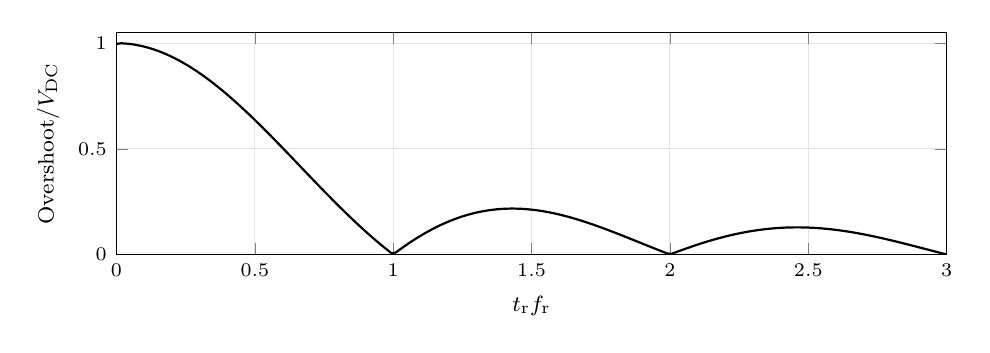
\begin{tikzpicture}
					\begin{axis}[
							width=\linewidth, height=4.4cm,
							xmin=0, xmax=3, ymin=0, ymax=1.05,
							xlabel={$t_\mathrm{r}f_\mathrm{r}$}, ylabel={Overshoot$/V_\mathrm{DC}$},
							grid=major, grid style={gray!20},
							tick label style={font=\scriptsize}, label style={font=\footnotesize},
						]
						\addplot[black, thick, domain=0.001:3, samples=200] {abs(sin(deg(pi*x)))/(pi*x)};
					\end{axis}
				\end{tikzpicture}
				\caption{Voltage step with a linear edge $t_\mathrm{r}$ into an undamped $LC$ circuit}
			\end{figure}
		\end{column}
		\begin{column}{0.49\textwidth}
			\small
			\textbf{Turn-on} of the other switch charges $C$ through $L_\mathrm{loop}$:
			\begin{itemize}
				\item step: up to $2V_\mathrm{DC}$, i.e.\ 100\,\% overshoot
				\item edges slower than $1/f_\mathrm{r}$ excite little ringing
			\end{itemize}
			\textbf{Turn-off} with current $I$: the loop current must stop.
			\begin{itemize}
				\item slow current fall $t_\mathrm{f}\gg1/f_\mathrm{r}$: $\Delta V\approx L_\mathrm{loop}I/t_\mathrm{f}$
				\item any speed (lossless bound): $\Delta V\leq I\,Z_0$
			\end{itemize}
			Measured on a 12\,V GaN buck: 100\,\% overshoot with $L_\mathrm{loop}=1.6$\,nH, 25\,\% with 0.4\,nH. For a fixed rating, overshoot limits the usable input voltage.
		\end{column}
	\end{columns}
	\blfootnote{Sources: Kassakian et al., Principles of Power Electronics, 2nd ed., 2023, Eq.\ (22.1); Reusch and Strydom, IEEE TPEL, 2014.}
\end{frame}

%%%%%%%%%%%%%%%%%%%%%%%%%%%%%%%%%%%%%%%%%%%%%%%%%%%%%%%%%%%%%
%% Your turn: ring and overshoot %%
%%%%%%%%%%%%%%%%%%%%%%%%%%%%%%%%%%%%%%%%%%%%%%%%%%%%%%%%%%%%%
% Two pages: task (page 1) and task with solution (page 2).
\begin{frame}<handout:1-2>
	\frametitle{Ring and overshoot}
	\begin{block}{Task (5 minutes)}
		A GaN half-bridge switches 10\,A at 48\,V. The switch-node voltage rings at 200\,MHz; the datasheet gives $C_\mathrm{oss}=250$\,pF at 48\,V.
		\begin{enumerate}
			\item Estimate the loop inductance.
			\item At turn-off the current falls at 10\,A/ns. Estimate the overshoot with $L\,\mathrm{d}i/\mathrm{d}t$ and with $I\,Z_0$. Which estimate applies?
			\item The switch-node edge at turn-on takes 1\,ns. The devices are rated 100\,V. Is there margin?
		\end{enumerate}
	\end{block}
	\onslide<2-|handout:2>{
		\small
		\begin{enumerate}
			\item $L_\mathrm{loop}=1/\big((2\pi f_\mathrm{r})^2C\big)=1/\big((2\pi\cdot200\,\mathrm{MHz})^2\cdot250\,\mathrm{pF}\big)=2.5$\,nH; ringing period $T_\mathrm{r}=5$\,ns.
			\item $L\,\mathrm{d}i/\mathrm{d}t=25$\,V; $Z_0=3.2\,\Omega$, $I Z_0=32$\,V. The current falls within 1\,ns, much faster than $T_\mathrm{r}$: the bound applies (undamped calculation: 30\,V). $L\,\mathrm{d}i/\mathrm{d}t$ holds only for $t_\mathrm{f}\gg T_\mathrm{r}$.
			\item $t_\mathrm{r}f_\mathrm{r}=0.2$: overshoot up to 94\,\% of 48\,V, i.e.\ a peak near 93\,V (no damping). No margin. A smaller $L_\mathrm{loop}$ raises $f_\mathrm{r}$ and lowers $Z_0$, which helps at both edges.
		\end{enumerate}
	}
\end{frame}

%%%%%%%%%%%%%%%%%%%%%%%%%%%%%%%%%%%%%%%%%%%%%%%%%%%%%%%%%%%%%
%% Energy in the loop inductance %%
%%%%%%%%%%%%%%%%%%%%%%%%%%%%%%%%%%%%%%%%%%%%%%%%%%%%%%%%%%%%%
\begin{frame}
	\frametitle{Loss caused by loop inductance}
	\begin{itemize}
		\item Turn-on: $L_\mathrm{loop}\,\mathrm{d}i/\mathrm{d}t$ lowers the switch voltage while the current rises; part of the turn-on loss is saved.
		\item Turn-off: $\frac12L_\mathrm{loop}I^2$ (100\,nJ for 2\,nH, 10\,A) is dissipated in the switch (slow turn-off) or in the ringing (fast turn-off).
	\end{itemize}
	\begin{table}
		\centering
		\small
		\begin{tabular}{|l|l|l|}
			\hline
			\textbf{Change}                                  & \textbf{Basis} & \textbf{Effect}                                   \\
			\hline
			$L_\mathrm{CS}=1$\,nH                            & calculated     & loss $+50$\,\%                                    \\
			$L_\mathrm{loop}=3$\,nH                          & calculated     & loss $+30$\,\%, partly saved at turn-on           \\
			$L_\mathrm{loop}$ from 0.4 to 2.9\,nH            & measured       & efficiency more than 4\,\% lower                 \\
			$L_\mathrm{loop}$ above 1.4\,nH                  & measured       & overshoot stops rising, switching slows down      \\
			\hline
		\end{tabular}
		\caption{eGaN buck converter 12\,V to 1.2\,V, 20\,A, 1\,MHz (Reusch and Strydom)}
	\end{table}
	\vspace{-0.6em}
	\begin{block}{Key message}
		A large loop inductance causes overshoot, slows the switching and costs efficiency.
	\end{block}
	\blfootnote{Sources: Reusch and Strydom, IEEE TPEL, 2014; on ringing loss: Zhang, Guo, Wang, IEEE TPEL, 2019.}
\end{frame}

%%%%%%%%%%%%%%%%%%%%%%%%%%%%%%%%%%%%%%%%%%%%%%%%%%%%%%%%%%%%%
%% Cgd coupling %%
%%%%%%%%%%%%%%%%%%%%%%%%%%%%%%%%%%%%%%%%%%%%%%%%%%%%%%%%%%%%%
\begin{frame}
	\frametitle{Coupling through $C_\mathrm{GD}$}
	\begin{columns}[T]
		\begin{column}{0.44\textwidth}
			\begin{figure}
				\centering
				\begin{circuitikz}[scale=0.7, transform shape]
					\draw (2.8,1.6) node[nigfete](Q){};
					\draw (Q.D) -- ++(0,0.6) coordinate (d0) -- ++(0,0.6) node[above]{$v_\mathrm{sw}$ rising};
					\draw (Q.S) -- ++(0,-0.6) coordinate (s0) -- ++(0,-0.4) coordinate (gnd) node[ground]{};
					\draw (Q.G) -- ++(-1.0,0) coordinate (g0);
					\draw (g0) to[C, l_=$C_\mathrm{GD}$, *-] (g0 |- d0) -- (d0);
					\draw (g0) to[C, l=$C_\mathrm{GS}$] (g0 |- s0) -- (s0);
					\draw (g0) to[R, l=$R_\mathrm{G,off}$] ++(-2.2,0) coordinate (dv) to[sV, l_=0\,V] (dv |- gnd) -- (gnd);
				\end{circuitikz}
				\caption{Low-side switch, off, while the high-side switch turns on}
			\end{figure}
		\end{column}
		\begin{column}{0.53\textwidth}
			\small
			The switch-node edge drives $i=C_\mathrm{GD}\,\mathrm{d}v/\mathrm{d}t$ into the gate loop:
			\begin{itemize}
				\item edge slow compared with $R_\mathrm{G,off}C_\mathrm{iss}$: $\Delta v_\mathrm{GS}\approx R_\mathrm{G,off}C_\mathrm{GD}\,\mathrm{d}v/\mathrm{d}t$
				\item voltage step (upper bound): $\Delta v_\mathrm{GS}=V_\mathrm{DC}\,C_\mathrm{GD}/(C_\mathrm{GD}+C_\mathrm{GS})$
			\end{itemize}
			Illustrative 650\,V GaN, $C_\mathrm{GD}=2$\,pF, $C_\mathrm{GS}=250$\,pF, $V_\mathrm{th}\approx1.5$\,V, 400\,V at 100\,V/ns:
			\begin{itemize}
				\item $R_\mathrm{G,off}=1\,\Omega$: 0.2\,V, safe
				\item step bound: 3.2\,V, false turn-on
			\end{itemize}
			The off path must keep a low impedance up to hundreds of MHz: short gate loop. Details in L4.
		\end{column}
	\end{columns}
\end{frame}

%%%%%%%%%%%%%%%%%%%%%%%%%%%%%%%%%%%%%%%%%%%%%%%%%%%%%%%%%%%%%
%% Layout rules %%
%%%%%%%%%%%%%%%%%%%%%%%%%%%%%%%%%%%%%%%%%%%%%%%%%%%%%%%%%%%%%
\subsection{Layout rules}

\begin{frame}
	\frametitle{Lateral, vertical and optimal loop}
	\begin{figure}
		\centering
		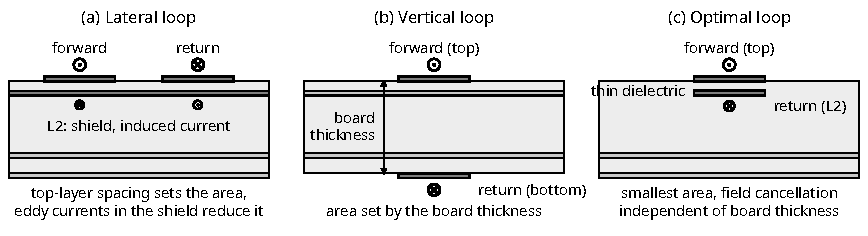
\includegraphics[width=0.92\linewidth]{fig/lec03/pcb_loop_sections.pdf}
		\caption{Cross-sections perpendicular to the loop current (schematic)}
	\end{figure}
	\vspace{-0.4em}
	\begin{table}
		\centering
		\footnotesize
		\begin{tabular}{|>{\raggedright\arraybackslash}p{5.3cm}|>{\raggedright\arraybackslash}p{3.7cm}|>{\raggedright\arraybackslash}p{3.7cm}|}
			\hline
			\textbf{Lateral}: no shield / shield at 0.66 / 0.33 / 0.1\,mm & \textbf{Vertical}: board 1.6 / 0.8\,mm & \textbf{Optimal}: return at 0.3 / 0.1\,mm \\
			3.92 / 2.74 / 2.10 / 1.36\,nH                                  & 2.87 / 1.83\,nH                         & 0.87 / 0.37\,nH                          \\
			\hline
		\end{tabular}
		\caption{Two 3\,mm $\times$ 8\,mm conductors, ideal end connections, FastHenry at 100\,MHz; same trends as in the measurements of Reusch and Strydom}
	\end{table}
\end{frame}

%%%%%%%%%%%%%%%%%%%%%%%%%%%%%%%%%%%%%%%%%%%%%%%%%%%%%%%%%%%%%
%% Optimal power loop %%
%%%%%%%%%%%%%%%%%%%%%%%%%%%%%%%%%%%%%%%%%%%%%%%%%%%%%%%%%%%%%
\begin{frame}
	\frametitle{Optimal power loop}
	\begin{columns}[T]
		\begin{column}{0.5\textwidth}
			\begin{table}
				\centering
				\footnotesize
				\begin{tabular}{|l|c|c|c|}
					\hline
					                                & \textbf{Lat.} & \textbf{Vert.} & \textbf{Opt.} \\
					\hline
					Parts on one side               & yes           & no             & yes           \\
					Field cancellation              & no            & yes            & yes           \\
					$L$ independent of thickness    & yes           & no             & yes           \\
					Shield layer needed             & yes           & no             & no            \\
					\hline
				\end{tabular}
				\caption{Properties of the three loop types}
			\end{table}
			\small
			Four-layer boards, 2\,oz copper (simulation and measurement):
			\begin{itemize}
				\item vertical: $L$ up to 80\,\% higher when the board thickness doubles from 0.8 to 1.6\,mm
				\item lateral: higher loss for the same $L$ (eddy currents in the shield)
			\end{itemize}
		\end{column}
		\begin{column}{0.46\textwidth}
			\small
			Optimal layout: input capacitors next to the drain of the high-side switch, return on the first inner layer directly underneath, rows of interleaved vias between the switches.
			\begin{itemize}
				\item 40\,\% lower loop inductance than the best conventional layout
				\item 35\,\% less overshoot, 10\,\% less loss
				\item full-load efficiency 0.8 and 1\,\% higher than with the vertical and lateral loop
			\end{itemize}
			Integration goes further: a monolithic GaN half-bridge reached about 0.15\,nH, the discrete design 0.25\,nH.
		\end{column}
	\end{columns}
	\blfootnote{Sources: Reusch and Strydom, IEEE TPEL, 2014; Lidow et al., 2019, Sec.\ 4.3, 4.4 and 10.2.}
\end{frame}

%%%%%%%%%%%%%%%%%%%%%%%%%%%%%%%%%%%%%%%%%%%%%%%%%%%%%%%%%%%%%
%% Return current path %%
%%%%%%%%%%%%%%%%%%%%%%%%%%%%%%%%%%%%%%%%%%%%%%%%%%%%%%%%%%%%%
\begin{frame}
	\frametitle{Return current path}
	\begin{columns}[T]
		\begin{column}{0.5\textwidth}
			\begin{figure}
				\centering
				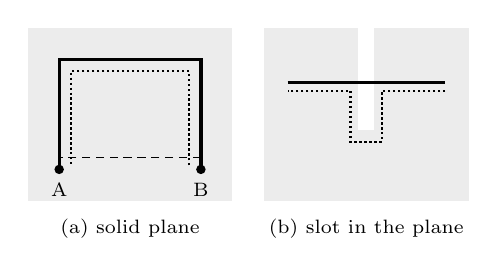
\begin{tikzpicture}[font=\scriptsize]
					% (a) plane with a U-shaped trace
					\fill[gray!15] (0,0) rectangle (2.6,2.2);
					\draw[very thick] (0.4,0.4) -- (0.4,1.8) -- (2.2,1.8) -- (2.2,0.4);
					\fill (0.4,0.4) circle (0.06); \fill (2.2,0.4) circle (0.06);
					\node[anchor=north] at (0.4,0.35) {A}; \node[anchor=north] at (2.2,0.35) {B};
					\draw[densely dashed] (2.2,0.55) -- (0.4,0.55);
					\draw[densely dotted, thick] (2.05,0.45) -- (2.05,1.65) -- (0.55,1.65) -- (0.55,0.45);
					\node at (1.3,-0.35) {(a) solid plane};
					% (b) plane with a slot under the trace
					\begin{scope}[xshift=3.0cm]
						\fill[gray!15] (0,0) rectangle (2.6,2.2);
						\fill[white] (1.2,0.9) rectangle (1.4,2.2);
						\draw[very thick] (0.3,1.5) -- (2.3,1.5);
						\draw[densely dotted, thick] (2.3,1.4) -- (1.5,1.4) -- (1.5,0.75) -- (1.1,0.75) -- (1.1,1.4) -- (0.3,1.4);
						\node at (1.3,-0.35) {(b) slot in the plane};
					\end{scope}
				\end{tikzpicture}
				\caption{Top view: trace (solid), return current at low (dashed) and high frequency (dotted)}
			\end{figure}
		\end{column}
		\begin{column}{0.47\textwidth}
			\small
			\begin{itemize}
				\item Low frequency: path of least resistance. High frequency: path of least inductance, under the trace. The transition lies at a few hundred kHz.
				\item Current density in the plane, conductor at height $h$:
				      \begin{equation*}
					      K(x)=\frac{I}{\pi h}\cdot\frac{1}{1+(x/h)^2}
				      \end{equation*}
				      50\,\% within $\pm h$, 80\,\% within $\pm3h$.
				\item A slot in the plane forces a detour: more inductance and radiation. No splits under high-frequency currents.
			\end{itemize}
		\end{column}
	\end{columns}
	\blfootnote{Source: Ott, 2009, Sec.\ 3.2; $K(x)$ from the image of the conductor in the plane.}
\end{frame}

%%%%%%%%%%%%%%%%%%%%%%%%%%%%%%%%%%%%%%%%%%%%%%%%%%%%%%%%%%%%%
%% Decoupling capacitors %%
%%%%%%%%%%%%%%%%%%%%%%%%%%%%%%%%%%%%%%%%%%%%%%%%%%%%%%%%%%%%%
\begin{frame}
	\frametitle{Decoupling capacitors}
	\begin{itemize}
		\item Place the high-frequency capacitors inside the power loop, at the drain of the high-side and the source of the low-side switch, on the same side as the switches.
		\item Use several equal capacitors in parallel, each with its own vias: $n$ capacitors give about $1/n$ of the inductance, and the current spreads over a wider path.
		\item Class II ceramics (X7R, X5R) lose a large part of their capacitance under DC bias. Use the DC-bias curve of the manufacturer, not the nominal value. C0G does not lose capacitance but has a low capacitance per volume.
		\item The ceramic capacitors supply the pulsed input current. Size them for ripple voltage and RMS current; the bulk capacitor covers low frequencies and the input filter.
	\end{itemize}
	\begin{block}{Example: buck 48\,V to 12\,V, 10\,A, 1\,MHz ($D=0.25$)}
		RMS current in the ceramic capacitors $I_\mathrm{o}\sqrt{D(1-D)}=4.3$\,A. For 1\,V ripple they need
		$C\geq I_\mathrm{o}D(1-D)/(\Delta V f_\mathrm{sw})=1.9\,\mu$F, effective at 48\,V, i.e.\ after the DC-bias derating.
	\end{block}
\end{frame}

%%%%%%%%%%%%%%%%%%%%%%%%%%%%%%%%%%%%%%%%%%%%%%%%%%%%%%%%%%%%%
%% Anti-resonance %%
%%%%%%%%%%%%%%%%%%%%%%%%%%%%%%%%%%%%%%%%%%%%%%%%%%%%%%%%%%%%%
\begin{frame}
	\frametitle{Bulk and ceramic capacitors}
	\begin{columns}[T]
		\begin{column}{0.52\textwidth}
			\begin{figure}
				\centering
				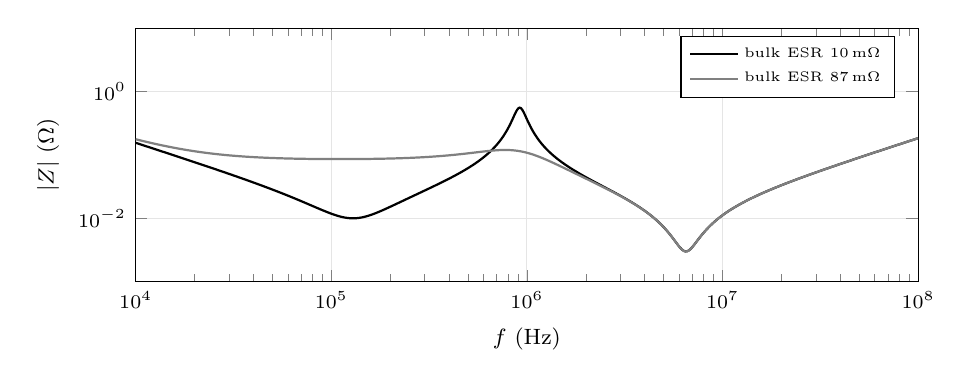
\begin{tikzpicture}[
						declare function={w(\x)=2*pi*10^\x;
								Xa(\x)=w(\x)*0.3e-9-1/(w(\x)*2e-6);
								Xb(\x)=w(\x)*15e-9-1/(w(\x)*100e-6);
								Zp(\x,\ra,\rb)=sqrt(((\ra*\rb-Xa(\x)*Xb(\x))^2+(\ra*Xb(\x)+\rb*Xa(\x))^2)/((\ra+\rb)^2+(Xa(\x)+Xb(\x))^2));}]
					\begin{loglogaxis}[
							width=0.95\linewidth, height=4.8cm,
							xmin=1e4, xmax=1e8, ymin=1e-3, ymax=10,
							xlabel={$f$ (Hz)}, ylabel={$|Z|$ ($\Omega$)},
							grid=major, grid style={gray!20},
							tick label style={font=\scriptsize}, label style={font=\footnotesize},
							legend style={font=\tiny}, legend pos=north east, legend cell align=left,
						]
						\addplot[black, thick, domain=4:8, samples=600] ({10^x}, {Zp(x,0.003,0.010)});
						\addlegendentry{bulk ESR 10\,m$\Omega$}
						\addplot[gray, thick, domain=4:8, samples=600] ({10^x}, {Zp(x,0.003,0.087)});
						\addlegendentry{bulk ESR 87\,m$\Omega$}
					\end{loglogaxis}
				\end{tikzpicture}
				\caption{2\,$\mu$F ceramic (0.3\,nH, 3\,m$\Omega$) in parallel with 100\,$\mu$F bulk (15\,nH including its connection)}
			\end{figure}
		\end{column}
		\begin{column}{0.45\textwidth}
			\small
			Between the two series resonances the ceramic branch is capacitive and the bulk branch inductive: parallel resonance (anti-resonance) at
			\begin{equation*}
				f_\mathrm{ar}\approx\frac{1}{2\pi\sqrt{L_\mathrm{bulk}C_\mathrm{cer}}}=0.92\,\mathrm{MHz}
			\end{equation*}
			Peak 0.56\,$\Omega$, right at a typical $f_\mathrm{sw}$.
			\begin{itemize}
				\item Damping: resistance of about $\sqrt{L_\mathrm{bulk}/C_\mathrm{cer}}=87$\,m$\Omega$ in the bulk branch (e.g.\ an electrolytic capacitor): peak 0.12\,$\Omega$.
				\item Check where $f_\mathrm{ar}$ lies relative to $f_\mathrm{sw}$ and its harmonics.
			\end{itemize}
		\end{column}
	\end{columns}
	\blfootnote{Source: Ott, 2009, Sec.\ 11.4.3 (largest peaks for values an order of magnitude or more apart); values illustrative.}
\end{frame}

%%%%%%%%%%%%%%%%%%%%%%%%%%%%%%%%%%%%%%%%%%%%%%%%%%%%%%%%%%%%%
%% Gate loop layout %%
%%%%%%%%%%%%%%%%%%%%%%%%%%%%%%%%%%%%%%%%%%%%%%%%%%%%%%%%%%%%%
\begin{frame}
	\frametitle{Gate loop layout}
	\begin{columns}[T]
		\begin{column}{0.45\textwidth}
			\begin{figure}
				\centering
				\begin{tikzpicture}[font=\scriptsize]
					% driver and transistor
					\draw (0,0.6) rectangle (1.2,2.0); \node[align=center] at (0.6,1.3) {gate\\driver};
					\draw[fill=gray!15] (2.8,0.2) rectangle (4.4,2.4); \node at (3.6,2.65) {GaN};
					% gate and Kelvin return as a pair
					\draw[very thick] (1.2,1.55) -- (2.8,1.55);
					\draw[very thick, gray] (1.2,1.15) -- (2.8,1.15);
					\node[anchor=south] at (2.0,1.6) {G};
					\node[anchor=north] at (2.0,1.1) {K};
					\draw[-{Latex[length=1.5mm]}] (1.6,1.68) -- (2.4,1.68);
					\draw[-{Latex[length=1.5mm]}] (2.4,1.02) -- (1.6,1.02);
					% driver supply capacitor
					\draw (0.25,0.6) -- (0.25,0.35); \draw (0.95,0.6) -- (0.95,0.35);
					\draw (0.1,0.35) -- (0.4,0.35); \draw (0.1,0.27) -- (0.4,0.27);
					\node[anchor=north] at (0.6,0.2) {$C_\mathrm{VDD}$ at the pins};
					% power current, orthogonal
					\draw[-{Latex[length=2mm]}, thick] (4.0,3.1) -- (4.0,-0.5);
					\node[anchor=west] at (4.1,-0.3) {power current};
				\end{tikzpicture}
				\caption{Top view of driver and transistor (schematic); G gate, K Kelvin source}
			\end{figure}
		\end{column}
		\begin{column}{0.52\textwidth}
			\small
			\begin{itemize}
				\item Driver within a few mm of the gate; gate and return as a pair (side by side or on adjacent layers).
				\item Return to the Kelvin-source pin (chip-scale GaN: the source pads closest to the gate). The gate loop then carries no power current.
				\item Gate loop perpendicular to the power loop, or with opposite currents.
				\item Driver supply capacitor directly at the driver pins.
				\item A small gate-loop inductance allows a small $R_\mathrm{G}$ without gate ringing: $R_\mathrm{G}\geq2\sqrt{L_\mathrm{G}/C_\mathrm{GS}}$ (L4).
			\end{itemize}
		\end{column}
	\end{columns}
	\blfootnote{Source: Lidow et al., 2019, Sec.\ 3.3 and 4.2.}
\end{frame}

%%%%%%%%%%%%%%%%%%%%%%%%%%%%%%%%%%%%%%%%%%%%%%%%%%%%%%%%%%%%%
%% Layer stack-up %%
%%%%%%%%%%%%%%%%%%%%%%%%%%%%%%%%%%%%%%%%%%%%%%%%%%%%%%%%%%%%%
\begin{frame}
	\frametitle{Layer stack-up}
	\begin{columns}[T]
		\begin{column}{0.55\textwidth}
			\begin{figure}
				\centering
				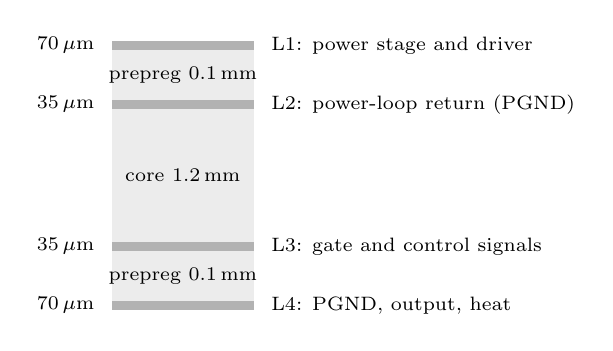
\begin{tikzpicture}[font=\scriptsize]
					% laminate (not to scale)
					\fill[gray!15] (0,0.12) rectangle (1.8,0.75);
					\fill[gray!15] (0,0.87) rectangle (1.8,2.55);
					\fill[gray!15] (0,2.67) rectangle (1.8,3.3);
					\foreach \y/\name/\cu in {3.3/{L1: power stage and driver}/70, 2.55/{L2: power-loop return (PGND)}/35, 0.75/{L3: gate and control signals}/35, 0.0/{L4: PGND, output, heat}/70} {
						\fill[gray!60] (0,\y) rectangle (1.8,\y+0.12);
						\node[anchor=west] at (1.9,\y+0.06) {\name};
						\node[anchor=east] at (-0.1,\y+0.06) {\cu\,$\mu$m};
					}
					\node at (0.9,2.98) {prepreg 0.1\,mm};
					\node at (0.9,1.71) {core 1.2\,mm};
					\node at (0.9,0.43) {prepreg 0.1\,mm};
				\end{tikzpicture}
				\caption{Example 4-layer stack-up, 1.6\,mm, symmetric (not to scale)}
			\end{figure}
		\end{column}
		\begin{column}{0.42\textwidth}
			\small
			\begin{itemize}
				\item Thin dielectric between L1 and L2: return of the power loop, reference of the gate loop.
				\item Signals on L3 have their own reference plane and are shielded from the switch node by L2.
				\item Symmetric build against warping; thick copper outside for current and heat.
				\item Six layers: a second ground plane and more room for control signals.
			\end{itemize}
			Ask the PCB manufacturer for standard prepreg thicknesses and copper weights; they set the loop inductance.
		\end{column}
	\end{columns}
\end{frame}

%%%%%%%%%%%%%%%%%%%%%%%%%%%%%%%%%%%%%%%%%%%%%%%%%%%%%%%%%%%%%
%% Switch-node copper %%
%%%%%%%%%%%%%%%%%%%%%%%%%%%%%%%%%%%%%%%%%%%%%%%%%%%%%%%%%%%%%
\begin{frame}
	\frametitle{Switch-node copper}
	\begin{columns}[T]
		\begin{column}{0.48\textwidth}
			\textbf{Small area}
			\begin{itemize}
				\item less capacitance to planes and heat sink: lower $\frac12CV^2f_\mathrm{sw}$ and common-mode current
				\item less coupling into gate and control signals
				\item 25\,mm$^2$ over L2 at 0.1\,mm are already 10\,pF
			\end{itemize}
		\end{column}
		\begin{column}{0.48\textwidth}
			\textbf{Large area}
			\begin{itemize}
				\item heat spreading for the high-side switch, whose source pad is the switch node
				\item lower resistance to the output inductor
			\end{itemize}
		\end{column}
	\end{columns}
	\vspace{0.4em}
	\begin{itemize}
		\item Output inductor right next to the switches.
		\item No ground or quiet copper under the switch node and the high-side driver, except the return plane under the power loop.
		\item Cool the high-side switch through thermal vias to a small pad on the bottom layer and an insulating thermal interface, or from the top of the package (top-cooled devices).
	\end{itemize}
	\blfootnote{Source: Lidow et al., 2019, Sec.\ 3.8 and 5.3 (about 10\,pF switch-node capacitance on their 48\,V boards).}
\end{frame}

%%%%%%%%%%%%%%%%%%%%%%%%%%%%%%%%%%%%%%%%%%%%%%%%%%%%%%%%%%%%%
%% Copper and spacing %%
%%%%%%%%%%%%%%%%%%%%%%%%%%%%%%%%%%%%%%%%%%%%%%%%%%%%%%%%%%%%%
\begin{frame}
	\frametitle{Copper and spacing}
	\begin{columns}[T]
		\begin{column}{0.48\textwidth}
			\textbf{Copper weight}
			\begin{table}
				\centering
				\footnotesize
				\begin{tabular}{|l|r|r|}
					\hline
					                      & 1\,oz    & 2\,oz    \\
					\hline
					Thickness             & 35\,$\mu$m & 70\,$\mu$m \\
					m$\Omega$ per square, 20\,$^\circ$C & 0.49 & 0.25 \\
					\hline
				\end{tabular}
			\end{table}
			Skin depth of copper: 66\,$\mu$m at 1\,MHz, 21\,$\mu$m at 10\,MHz, 6.6\,$\mu$m at 100\,MHz. Thicker copper helps the DC and low-frequency current, not the ringing current. Current capacity versus temperature rise: IPC-2152.
		\end{column}
		\begin{column}{0.48\textwidth}
			\textbf{Spacing}
			\begin{table}
				\centering
				\footnotesize
				\begin{tabular}{|l|r|r|}
					\hline
					Conductor spacing        & 31--50\,V & 301--500\,V \\
					\hline
					internal layers          & 0.1\,mm   & 0.25\,mm \\
					external, uncoated       & 0.6\,mm   & 2.5\,mm  \\
					external, coated         & 0.13\,mm  & 0.8\,mm  \\
					\hline
				\end{tabular}
				\caption{Minimum spacing, IPC-2221 (rev.\ B), Tab.\ 6-1}
			\end{table}
			These are functional spacings. Mains-connected products need creepage and clearance for basic or reinforced insulation (IEC 62368-1, IEC 60664-1), which are much larger.
		\end{column}
	\end{columns}
\end{frame}

%%%%%%%%%%%%%%%%%%%%%%%%%%%%%%%%%%%%%%%%%%%%%%%%%%%%%%%%%%%%%
%% Damping and snubbers %%
%%%%%%%%%%%%%%%%%%%%%%%%%%%%%%%%%%%%%%%%%%%%%%%%%%%%%%%%%%%%%
\subsection{Damping and snubbers}

\begin{frame}
	\frametitle{RC snubber}
	\begin{columns}[T]
		\begin{column}{0.48\textwidth}
			\begin{figure}
				\centering
				\begin{tikzpicture}
					\begin{semilogxaxis}[
							width=\linewidth, height=4.5cm,
							xmin=0.1, xmax=10, ymin=0, ymax=1.05,
							xlabel={$R/Z_0$}, ylabel={Damping ratio $\zeta$},
							grid=major, grid style={gray!20},
							tick label style={font=\scriptsize}, label style={font=\footnotesize},
							legend style={font=\tiny}, legend pos=north east, legend cell align=left,
						]
						\addplot[black, thick] table[x=r, y=n10] {fig/lec03/snubber_damping.dat};
						\addlegendentry{$C_\mathrm{s}=10\,C_\mathrm{par}$}
						\addplot[black, thick, dashed] table[x=r, y=n3] {fig/lec03/snubber_damping.dat};
						\addlegendentry{$C_\mathrm{s}=3\,C_\mathrm{par}$}
						\addplot[gray, thick] table[x=r, y=n1] {fig/lec03/snubber_damping.dat};
						\addlegendentry{$C_\mathrm{s}=C_\mathrm{par}$}
					\end{semilogxaxis}
				\end{tikzpicture}
				\caption{Damping of the ring by $R$ and $C_\mathrm{s}$ in series across the switch}
			\end{figure}
		\end{column}
		\begin{column}{0.49\textwidth}
			\small
			\begin{enumerate}
				\item Measure the ring $f_\mathrm{r0}$; add a known $C_\mathrm{add}$ across the switch and measure $f_\mathrm{r1}$:
				      \begin{equation*}
					      C_\mathrm{par}=\frac{C_\mathrm{add}}{(f_\mathrm{r0}/f_\mathrm{r1})^2-1},\quad L=\frac{1}{(2\pi f_\mathrm{r0})^2C_\mathrm{par}}
				      \end{equation*}
				      The frequency halves for $C_\mathrm{add}=3C_\mathrm{par}$.
				\item $R\approx Z_0=\sqrt{L/C_\mathrm{par}}$ and $C_\mathrm{s}\approx3$--$4\,C_\mathrm{par}$ give $\zeta\approx0.5$--0.6.
				\item Added loss: $\frac12C_\mathrm{s}V^2$ per fast edge, at most $C_\mathrm{s}V^2f_\mathrm{sw}$.
			\end{enumerate}
			Small packages for $R$ and $C_\mathrm{s}$, inside the power loop; otherwise their own inductance makes them useless at $f_\mathrm{r}$.
		\end{column}
	\end{columns}
	\blfootnote{Sources: Taylor and Manack, TI SLYT465, 2012; damping curves computed for this lecture.}
\end{frame}

%%%%%%%%%%%%%%%%%%%%%%%%%%%%%%%%%%%%%%%%%%%%%%%%%%%%%%%%%%%%%
%% Snubber or layout %%
%%%%%%%%%%%%%%%%%%%%%%%%%%%%%%%%%%%%%%%%%%%%%%%%%%%%%%%%%%%%%
% Two pages: task (page 1) and task with solution (page 2).
\begin{frame}<handout:1-2>
	\frametitle{Snubber or layout?}
	\begin{block}{Task (4 minutes)}
		The half-bridge of the earlier task (48\,V, 1\,MHz, $C_\mathrm{par}=250$\,pF) has been improved to $L_\mathrm{loop}=1$\,nH.
		\begin{enumerate}
			\item Design an RC snubber with $C_\mathrm{s}=3\,C_\mathrm{par}$.
			\item What does it cost? Compare with the energy $\frac12 L_\mathrm{loop}I^2$ at 10\,A.
		\end{enumerate}
	\end{block}
	\onslide<2-|handout:2>{
		\small
		\begin{enumerate}
			\item $Z_0=\sqrt{1\,\mathrm{nH}/250\,\mathrm{pF}}=2\,\Omega$, so $R=2\,\Omega$ and $C_\mathrm{s}=750$\,pF.
			\item Added loss between $\frac12C_\mathrm{s}V^2f_\mathrm{sw}=0.86$\,W and $C_\mathrm{s}V^2f_\mathrm{sw}=1.7$\,W. The ring itself carries only $\frac12LI^2=50$\,nJ, i.e.\ 0.05\,W at 1\,MHz.
		\end{enumerate}
		\begin{block}{Conclusion}
			At MHz switching a full snubber costs more than the ringing. First reduce $L_\mathrm{loop}$, then accept some ringing, and use a small snubber only where overshoot or EMI demand it.
		\end{block}
	}
\end{frame}

%%%%%%%%%%%%%%%%%%%%%%%%%%%%%%%%%%%%%%%%%%%%%%%%%%%%%%%%%%%%%
%% Ringing demo %%
%%%%%%%%%%%%%%%%%%%%%%%%%%%%%%%%%%%%%%%%%%%%%%%%%%%%%%%%%%%%%
\begin{frame}
	\frametitle{Two loop inductances}
	\begin{columns}[T]
		\begin{column}{0.55\textwidth}
			\begin{figure}
				\centering
				\begin{tikzpicture}
					\begin{axis}[
							width=\linewidth, height=5.0cm,
							xmin=-1, xmax=10, ymin=-5, ymax=90,
							xlabel={$t$ (ns)}, ylabel={$v_\mathrm{sw}$ (V)},
							grid=major, grid style={gray!20},
							tick label style={font=\scriptsize}, label style={font=\footnotesize},
							legend style={font=\tiny}, legend pos=north east, legend cell align=left,
						]
						\addplot[gray, thick] table[x=t, y=v04] {fig/lec03/ring_turn_on.dat};
						\addlegendentry{0.4\,nH}
						\addplot[black, thick] table[x=t, y=v16] {fig/lec03/ring_turn_on.dat};
						\addlegendentry{1.6\,nH}
					\end{axis}
				\end{tikzpicture}
				\caption{Model of the hard turn-on: 48\,V, $C=260$\,pF, $t_\mathrm{r}=1$\,ns, $Q=8$}
			\end{figure}
		\end{column}
		\begin{column}{0.42\textwidth}
			\small
			Same edge, two layouts:
			\begin{itemize}
				\item 0.4\,nH: 494\,MHz, peak 73\,V
				\item 1.6\,nH: 247\,MHz, peak 84\,V
			\end{itemize}
			The smaller loop rings at twice the frequency with less overshoot, because the 1\,ns edge is half a ringing period long.\\[0.4em]
			Demo: measure the ring of a GaN half-bridge with a probe of at least 1\,GHz bandwidth and a short ground spring, and compare it with this model (notebook of Tutorial 3).
		\end{column}
	\end{columns}
\end{frame}

%%%%%%%%%%%%%%%%%%%%%%%%%%%%%%%%%%%%%%%%%%%%%%%%%%%%%%%%%%%%%
%% Key messages %%
%%%%%%%%%%%%%%%%%%%%%%%%%%%%%%%%%%%%%%%%%%%%%%%%%%%%%%%%%%%%%
\begin{frame}
	\frametitle{Key messages}
	\begin{enumerate}
		\item The loop inductance is set by the area between forward and return current. Put the return on the adjacent layer, 0.1\,mm below the power loop.
		\item Hand formulas give the right order of magnitude; a field solver gives the value of the routed layout.
		\item $L_\mathrm{loop}$ and $C_\mathrm{oss}+C_\mathrm{par}$ ring at hundreds of MHz. Overshoot is at most $IZ_0$ at turn-off and $V_\mathrm{DC}$ at turn-on.
		\item Common-source inductance and $C_\mathrm{GD}$ couple the power loop into the gate loop: Kelvin source, short gate loop.
		\item Capacitance $C$ at the switch node costs $\frac12CV^2f_\mathrm{sw}$ in hard switching and carries $C\,\mathrm{d}v/\mathrm{d}t$ as common-mode current.
		\item At MHz, a better layout is cheaper than a snubber.
	\end{enumerate}
\end{frame}

%%%%%%%%%%%%%%%%%%%%%%%%%%%%%%%%%%%%%%%%%%%%%%%%%%%%%%%%%%%%%
%% Exit ticket %%
%%%%%%%%%%%%%%%%%%%%%%%%%%%%%%%%%%%%%%%%%%%%%%%%%%%%%%%%%%%%%
% Two pages: questions (page 1) and answers (page 2).
\begin{frame}<handout:1-2>
	\frametitle{Exit ticket}
	\begin{varblock}[\textwidth]{Three questions, one minute each}
		\begin{enumerate}
			\item Which change lowers the loop inductance most: 2\,oz instead of 1\,oz copper, twice the trace width, or the return on L2 instead of L4?
			\item The ringing frequency rises from 200 to 400\,MHz after a layout change, with the same devices. By which factor did $L_\mathrm{loop}$ change?
			\item Why is a large switch-node copper area a problem at 400\,V?
		\end{enumerate}
	\end{varblock}
	\onslide<2-|handout:2>{
		\begin{enumerate}
			\item The return on L2: the spacing drops from about 1.6\,mm to 0.1\,mm. Twice the width roughly halves $L$; the copper thickness hardly matters.
			\item $f_\mathrm{r}\propto1/\sqrt{L}$: four times lower.
			\item Its capacitance adds $\frac12CV^2f_\mathrm{sw}$ of hard-switching loss and $C\,\mathrm{d}v/\mathrm{d}t$ of common-mode current, both large at high voltage.
		\end{enumerate}
	}
\end{frame}

%%%%%%%%%%%%%%%%%%%%%%%%%%%%%%%%%%%%%%%%%%%%%%%%%%%%%%%%%%%%%
%% References %%
%%%%%%%%%%%%%%%%%%%%%%%%%%%%%%%%%%%%%%%%%%%%%%%%%%%%%%%%%%%%%
\begin{frame}
	\frametitle{References}
	\scriptsize
	\begin{itemize}
		\item D. Reusch, J. Strydom, ``Understanding the effect of PCB layout on circuit performance in a high-frequency gallium-nitride-based point of load converter,'' IEEE Trans.\ Power Electron., vol.\ 29, no.\ 4, pp.\ 2008--2015, 2014.
		\item A. Lidow, M. de Rooij, J. Strydom, D. Reusch, J. Glaser, \textit{GaN Transistors for Efficient Power Conversion}, 3rd ed., Wiley, 2019, Ch.\ 3--5 and 10.
		\item H.\,W. Ott, \textit{Electromagnetic Compatibility Engineering}, Wiley, 2009, Ch.\ 3, 11 and App.\ E.
		\item Z. Zhang, B. Guo, F. Wang, L.\,M. Tolbert, B.\,J. Blalock, Z. Liang, P. Ning, ``Methodology for switching characterization evaluation of wide band-gap devices in a phase-leg configuration,'' IEEE APEC 2014, pp.\ 2534--2541.
		\item Z. Zhang, B. Guo, F. Wang, ``Evaluation of switching loss contributed by parasitic ringing for fast switching wide band-gap devices,'' IEEE Trans.\ Power Electron., vol.\ 34, no.\ 9, pp.\ 9082--9094, 2019.
		\item J.\,G. Kassakian, D.\,J. Perreault, G.\,C. Verghese, M.\,F. Schlecht, \textit{Principles of Power Electronics}, 2nd ed., Cambridge University Press, 2023, Ch.\ 22 and 24.
		\item E. Bogatin, \textit{Signal and Power Integrity -- Simplified}, 3rd ed., Pearson, 2018.
		\item M. Kamon, M.\,J. Tsuk, J.\,K. White, ``FASTHENRY: A multipole-accelerated 3-D inductance extraction program,'' IEEE Trans.\ Microw.\ Theory Techn., vol.\ 42, no.\ 9, pp.\ 1750--1758, 1994.
		\item R. Taylor, R. Manack, ``Controlling switch-node ringing in synchronous buck converters,'' TI Analog Applications Journal, SLYT465, 2012.
		\item IPC-2221B, \textit{Generic Standard on Printed Board Design}; IPC-2152, \textit{Standard for Determining Current Carrying Capacity in Printed Board Design}.
	\end{itemize}
\end{frame}
